
% Take extra care in avoiding ``expansion'' -- stick to ``evaluation''

\todo{Tie-breaking or tie-breaking? Tie-Breaking.}
%\todo{Inadmissible or non-admissible? Inadmissible.}
\todo{last frontier or final frontier?}

\begin{abstract}
% this current version is intentionally ambiguous as possible
Despite recent improvements in search techniques
for cost-optimal classical planning, the exponential growth of
the size of the search frontier in A* is unavoidable.
We investigate tie-breaking strategies for A*, 
experimentally analyzing the performance of standard tie-breaking strategies that break ties according to the heuristic value of the nodes.
We find that tie-breaking has a significant impact on search algorithm performance when there are zero-cost operators that induce large plateau regions in the search space.
We develop a new framework for tie-breaking based on a depth metric which measures distance from the entrance to the plateau, and propose a new, randomized strategy which significantly outperforms standard strategies on both existing planning benchmark domains and newly generated domains with zero-cost actions.

%%  % 
%% We investigate various existing myth on tie-breaking
%% strategies and propose simple yet effective methods for improving the
%% search performance within plateau.
%%  % 
%%  % 
%%  They do not depend on any particular heuristic, nor
%%  on multi-heuristic portfolio.
%%  They work even if the heuristic
%%  function no longer provides useful information.
%%  % Moreover, they do not even try to obtain any further information from
%%  % the domain.
%%  We empirically evaluate our strategies against state-of-the-art admissible planner.
\end{abstract}

\section{Introduction}
%Motivation: The Importance of the Last Frontier in A* and Domains with Large Plateaus
\label{sec-1}

%\subsubparagraph{\astar and perfect heuristics}

This paper investigates tie-breaking strategies for \astar.
\astar is a standard search algorithm for finding an optimal-cost path 
from an initial state $s$ to some goal state $g \in G$ in a search space represented as a graph \cite{hart1968formal}.
In each iteration, \astar selects and \emph{expands} a node $n$ from the OPEN priority queue.
$n$ is the node which has the lowest $f$-cost in OPEN, where for node $n$, $f(n)$ is the sum of  $g(n)$, the cost of the current path from the start state to $n$, and $h(n)$, a heuristic estimate of the cost from $n$ to a goal state.
\astar returns an optimal solution when $h$ is admissible, i.e., when $h \leq h^*$, where $h^*$ is the true distance to the goal.


In order to guarantee solution optimality, \astar expands all
nodes with $f(n) < f^*$, where $f^*$ is the cost of the optimal solution.
%All nodes with $f(n) = k$ are expanded before any node with $f(n) > k$ are expanded.
%Thus, after all nodes with $f(n) < f^*$ have been expanded, 
\astar expands \emph{some} of the nodes with $f(n) = f^*$, and never expands a node with $f(n) > f^*$.
Thus, the \emph{effective search space of \astar} is the set of nodes with 
$f(n) \leq f^*$, and
much of the work in the search and planning literature  has focused
on reducing the size of this effective search space by
developing more accurate, admissible heuristic functions.

In many problems, the size of the \emph{last frontier}, the set of nodes with $f(n)=f^*$, accounts for a significant fraction of the effective search space of \astar.
\refig{fig:plateau-noh} plots the \# of states with $f(n) = f^*$ (y-axis)
vs. the \# of states with $f(n) \leq f^*$
for 1104 problem instances from the International Planning Competition (IPC1998-2011).
For many instances,  a large fraction of the nodes with $f(n) \leq f^*$ have $f(n)=f^*$.
For example, in the \pddl{Openstacks} domain, almost all states with $f(n) \leq f^*$ have cost $f^*$.
In such domains, the tie-breaking policy which decides which nodes to expand in the last frontier can have a significant impact on the performance of \astar.

\begin{figure*}[bt]
 \newcommand{\minilength}{0.36\textwidth}
 \newcommand{\minisep}{0.02\textwidth}
 \begin{minipage}[t]{\minilength}
  \centering
 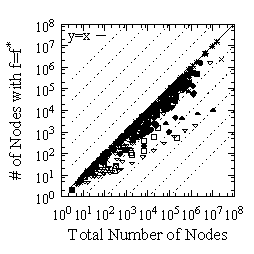
\includegraphics{tables/aaai16-frontier/aaai16prelim3/lmcut_frontier_noh-front-mono.pdf}
 \caption{
 The \# of nodes with $f=f^*$ (y-axis) compared to the
 total \# of nodes in the search space (x-axis) with $f\leq f^*$ on 1104 IPC benchmark problems
  (search space analyzed using modified Fast Downward with \lmcut heuristic which 
  generates all nodes with cost $f^*$).
  Dotted lines represent $\times 10^n$ boundaries.
  }
 \label{fig:plateau-noh}
 \end{minipage}
 \hfill
 \begin{minipage}[t]{\minilength}
  \centering
  % 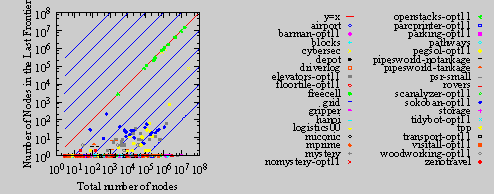
\includegraphics{tables/aaai16-frontier/aaai16prelim3/lmcut_frontier-front.pdf}
  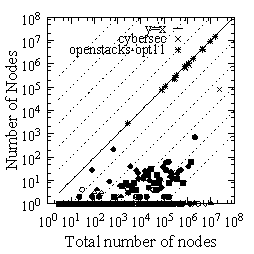
\includegraphics{tables/aaai16-frontier/aaai16prelim3/lmcut_frontier-front-mono.pdf}
  \caption{
  Similar to \refig{fig:plateau-noh}; $y$-axis is
  \# nodes with $[f,h]=[f^*,0]$, which forms the final
  plateau when $h$ tie-breaking is enabled.
  Many \pddl{Openstacks} and \pddl{Cybersec} are instances near the $y=x$ line.
  Due to space, We do not show all labels
  for point types. See supplement for a larger, fully
  labelled, colored version.
  }
  \label{plateau}
 \end{minipage} 
 \hfill
 \begin{minipage}[t]{0.23\textwidth}
  \centering
  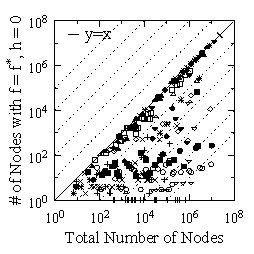
\includegraphics{tables/aaai16-frontier/zerocost/lmcut_frontier-front-mono.pdf}
  \caption{Similar to \refig{plateau}, but for 640 instances from our cost-minimization
  \emph{zerocost domains} (\refsec{sec:zerocost-domains}).
  Zero-cost actions induce very large plateau regions.
%  Even with $h$ tie-breaking, these domains force the planner
%  to search much larger plateau.
 }
 \label{plateau-zerocost}
 \end{minipage} 
\end{figure*}

In this paper, we investigate \emph{tie-breaking} strategy used by
\astar, which selects a node to expand among nodes with the same
$f$-cost.  
%Since \astar expands all nodes with $f$-cost less than $f^*$
%before expanding any nodes with cost $f^*$, the tie-breaking policy only
%affects performance when considering the last frontier (nodes with cost
%$f^*$).  Although there has not been much previous \emph{in-depth} work
%on tie-breaking policies for admissible search algorithms, 
It is widely believed that among nodes with
cost $f(n) = f^*$, ties should be broken according to $h(n)$, i.e.,
nodes with smaller $h$-values should be expanded first.  While this is a
useful rule of thumb in many domains, it turns out that tie-breaking
requires more careful consideration, particularly for problems with
large \emph{plateaus} -- regions of the search space with the same $f$ and $h$.
\emph{All tie-breaking strategies in this paper
maintain the admissibility of the search because they only affect node expansion
order among the nodes with the same $f$-cost.}

We first empirically evaluate standard tie-breaking strategies for \astar, and show that 
% 
(1) a Last-In-First-Out (\lifo) policy for tends to be more efficient than an a First-In-First-Out (\fifo) policy, and 
% 
(2) tie-breaking according to the heuristic value $h$, which
frequently appears in the heuristic search literature, has little 
impact on the performance as long as a \lifo policy is used.
% 
%% Remove?
% \todo[
% Third, the \lifo-based bucket implementation and $h$-based tie-breaking
% both share the greedy search pattern within the plateau of the
% search space.]{this is not shown yet. how to show it? xy-plot of the node
% evaluation order?}
These experiments show that there are significant performances differences among tie-breaking strategies
when domains include zero-cost actions.  While there are relatively few domains with zero-cost actions in the existing IPC benchmark sets, we argue that this is a historical accident, and that in fact, many unit-cost domains may be more appropriately modelled using zero-cost actions.
%Through these experiments, we points out a bias in the current set of
%benchmark domains and the importance of tie-breaking in
%the more practical cost-minimization problems.

In order to solve such problems more efficently,
we propose 
tie-breaking methods
based on a notion of \emph{depth} within the plateau, which corresponds to the number of steps 
a node is from the ``entrance'' to the plateau region, and show that a randomized, depth-based strategy
significantly outperforms 
other tie-breaking strategies using the same heuristic function.
Although depth-based tie-breaking is part of a multi-level tie-breaking strategy,
and we show that the notion of depth is the principal factor in determining performance.
Finally, we show the robustness of our tie-breaking strategies
against a particular action ordering in the domain definition.


% XXX It's doubtful that anybody would believe that machine-level efficiency of LIFO (compared to FIFO) is important in domain-independent planning.
%At the same time, we show that 
%the performance of above \lifo tie-breaking can be explained by its
%depth-first strategy, and the other characteristics of \lifo such as
%machine-level efficiency have little effect on the performance.

%% Above describes the enough detail of the paper structure?


\section{Preliminaries}

We first define some notation and terminology used throughout the rest of the paper.
A \emph{tie-breaking strategy} selects from among nodes with the same $f$-value.
Tie-breaking strategies are denoted as $[\text{criterion}_1, \text{criterion}_2, ..., \text{criterion}_k]$,
which means: If there multiple nodes with the same $f$-vaue, first, break ties using $\text{criterion}_1$. 
If there still multiple nodes remaining, then break ties using $\text{criterion}_2$ and so on, until a single node is selected.
The \emph{first-level tie-breaking policy} of a strategy is
$\text{criterion}_1$, the \emph{second-level tie-breaking policy} is
$\text{criterion}_2$, and so on.
%% the word frontier is no longer used in the later text.
% \emph{Last frontier} is the set of open nodes with $f^*$.
\emph{Plateau} is the set of open nodes with the same $f$ and same $h$.

In our experiments, all planners are based on Fast Downward (revision 6251), and all
experiments are run with a 5-minute, 2GB memory limit for the search binary (FD translation/preprocessing times are not included in the 5-minute limit).
All experiments were conducted on Xeon E5410@2.33GHz CPUs.
Our experimental results include 35 standard benchmark domains with 1104
problems and 29 \emph{zero-cost-action} domains with 640 problems, which is
described later.

\section{Background: Tie-breaking Strategies in \astar}

%Aside from the heuristic function, most best-first family of search
%algorithms, including \astar, IDA* and so on, have a tie-breaking criteria which is used
%when two nodes have the same $f$ value.

If multiple nodes with the same $f$-cost are possible, \astar
must implement some tie-breaking policy (either
explicitly or implicitly) which selects from among these nodes.
The early literature on heuristic search seems to have been mostly agnostic regarding tie-breaking.
The original \astar paper, 
%as well as Nilsson's subsequent textbook 
states: ``Select the open node $n$ whose value $f$
is smallest. Resolve ties arbitrarily, but always in favor of any [goal
node]'' \cite[p.102 Step 2]{hart1968formal} %\cite[p.69]{Nilsson71}.
% Although it is possible to interpret this to imply $h$-based tie-breaking
% since goal nodes are the special case where $h=0$,
% they make no further metion of tie-breaking.
Pearl's textbook on heuristic search specifies that best-first search should ``break ties arbitrarily'' (\citeyear{pearl1984heuristics}, p.48, Step 3), and does not specifically mention tie-breaking for \astar.
The first explicit mention of a tie-breaking policy that considers node generation order is by Korf in his analysis of IDA*: ``If \astar employs the tie-breaking rule of 'most-recently generated', it must also expand the same nodes [as IDA*]'', i.e., a \lifo ordering.

In recent years, tie-breaking accoording to $h$-values has become ``folklore'' in the search community.
\citeauthor{hansen2007anytime} state that ``It is well-known 
that \astar achieves best performance when it breaks ties
in favor of nodes with least h-cost'' \cite{hansen2007anytime}.
\citeauthor{holte2010common} writes ``\astar breaks ties in favour
of larger g values, as is most often done'' \cite[note that since $f=g+h$,
preferring large $g$ is equivalent to preferring smaller $h$]{holte2010common}.
% \citeauthor{felner2011inconsistent} also assume ``ties are broken in
% favor of low h-values'' in describing Bidirectional Pathmax for \astar.
In their detailed survey/tutorial on efficient \astar implementations,
\citeauthor{burns2012implementing} (\citeyear{burns2012implementing})
also break ties ``preferring high $g$.''
%% this could be moved to later analysis
% They further write: ``The reasoning is that the goal can be found more
% quickly in the final $f$ layer of search''.
Thus, tie-breaking according to $h$-values appears
to be ubiquitous in practice.
To our knowledge, there has never been an in-depth, experimental analysis of tie-breaking strategies for \astar.

Although the standard practice of tie-breaking according to $h$ might be
sufficient in some domains, further levels of tie-breaking (explicit or
implicit) are required if multiple nodes can have the same $f$ and
$h$ values.
%% we do, in Roger, Helmert 
% We are not aware of any work that explicitly mentions 2nd-level tie-breaking.
While the survey of efficient \astar implementation techniques in
\citeauthor{burns2012implementing} did not explicitly mention 2nd-level
tie-breaking, their code \cite{burnscode} first breaks ties according to $h$, and then
breaks remaining ties according to a \lifo policy (most recently
generated nodes first), i.e., a $[h,\lifo]$ strategy.
Although not documented, their choice of a \lifo 2nd-level tie-breaking policy appears to be a natural consequence of the fact it can be trivially, efficiently implemented in their two-level bucket (vector) implementation of OPEN.
In contrast, the current implementation of \sota \astar based planner Fast
Downward \cite{Helmert2006}, %\footnote{http://www.fast-downward.org}, <-- takes up 2 lines!
as well as 
the work by \cite{RogerH10} uses a $[h,\fifo]$ tie-breaking strategy.
Although we could not find an explanation, this choice is most likely due to their use of alternating OPEN lists, in which case the \fifo second-level policy serves to provide a limited form of fairness.
%We could not find any explanation for this choice either.


%\citeauthor{Korf1985depth} uses $h$-based tie-breaking in the context of WA*
%\cite{korf1993linear}.  
% ** not sure how/where to put this..

\section{Evaluation of  Standard Strategies}
\label{sec:eval-common-strategies}

We first compared two commonly used tie-breaking strategies $[h,\fifo]$, $[h,\lifo]$, which
first breaks ties according to $h$, and then applies \fifo or \lifo
second-level tie-breaking, respectively.
% The following will be necessary in a future version, if we use LOP:
%Although the search behavior of $[f,h,\fifo]$ corresponds to the default behavior of Fast Downward, this implementation differs 
%from the original, unmodified code because we enabled caching of $h$-values, so that reopened nodes refer to cached $h$-values.\footnote{The current Fast Downward code disables $h$-caching because its current implementation is not compatible with multiple admissible heuristics.}
%Thus, we also show results for unmodified Fast Downward -- as expected, $[f,h,\fifo]$ dominates unmodified FD.
Results for the LM-cut heuristic \cite{Helmert2009} are
shown in \reftbl{single-coverage} (Left).
Differences in coverage are observed in several domains.
Due to space limitation, we show only the domains
where there was any difference. Full data is available in the
supplemental material. 
% 
\refig{f-h-eval} gives us a
more fine-grained analysis by comparing the number of node evaluation
(computations of \lmcut) on different tie-breakings.


\begin{table}[tb]
 \centering \relsize{-3}
 \begin{tabular}{|c|c|c|}
\hline      
 Domain & \rotatebox[origin=l]{90}{${\mbox{lmcut}}_{\mbox{ff}}$}   & \rotatebox[origin=l]{90}{${\mbox{lmcut}}_{\mbox{lf}}$}    \\
\hline      
 sum(1104) &  558 &  \textbf{565}  \\
\hline      
 {\relsize{-1}airport(50)} &  \textbf{27} &  26  \\
 {\relsize{-1}cybersec(19)} &  2 &  \textbf{3}  \\
 {\relsize{-1}mystery(30)} &  15 &  \textbf{16}  \\
 {\relsize{-1}openstacks-opt11(20)} &  11 &  \textbf{18}  \\
 {\relsize{-1}pipesworld-notankage(50)} &  \textbf{15} &  14 \\
\hline
\end{tabular}

 \begin{tabular}{|c|c|c|}
\hline      
 Domain & \rotatebox[origin=l]{90}{ff,noh}   & \rotatebox[origin=l]{90}{lf,noh}    \\
\hline      
 sum(1104) &  442 &  \textbf{556}  \\
\hline      
 {\relsize{-1}airport(50)} &  18 &  \textbf{26}  \\
 {\relsize{-1}cybersec(19)} &  0 &  \textbf{3}  \\
 {\relsize{-1}driverlog(20)} &  12 &  \textbf{13}  \\
 {\relsize{-1}elevators-opt11(20)} &  14 &  \textbf{15}  \\
 {\relsize{-1}freecell(80)} &  8 &  \textbf{9}  \\
 {\relsize{-1}logistics00(28)} &  16 &  \textbf{18}  \\
 {\relsize{-1}miconic(150)} &  68 &  \textbf{140}  \\
 {\relsize{-1}mprime(35)} &  19 &  \textbf{22}  \\
 {\relsize{-1}nomystery-opt11(20)} &  12 &  \textbf{13}  \\
 {\relsize{-1}openstacks-opt11(20)} &  11 &  \textbf{18}  \\
 {\relsize{-1}parcprinter-opt11(20)} &  12 &  \textbf{13}  \\
 {\relsize{-1}pathways(30)} &  4 &  \textbf{5}  \\
 {\relsize{-1}pipesworld-tankage(50)} &  7 &  \textbf{8}  \\
 {\relsize{-1}scanalyzer-opt11(20)} &  4 &  \textbf{10}  \\
 {\relsize{-1}visitall-opt11(20)} &  9 &  \textbf{10}  \\
 {\relsize{-1}woodworking-opt11(20)} &  6 &  \textbf{9}  \\
 {\relsize{-1}zenotravel(20)} &  9 &  \textbf{11} \\
\hline
\end{tabular}

 \caption{Experiments with 5 min, 2GB setting,
 comparing the coverages of \fifo and \lifo
 tie-breaking, with (left) and without (right) the
 conventional first-level $h$-based tie-breaking.  Due to space, 
only domains with results that differ are shown.
(Full results are
 available in the supplemental material.)
 % \textbf{Boldface} denotes the case
 % where it achieved the best result among configurations.
 }
 \label{single-coverage}
\end{table}


\begin{figure}[tb]
 \centering \relsize{-3}
 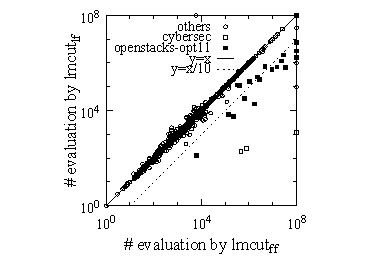
\includegraphics{tables/aaai16-30min-5min-cut/aaai16prelim3/evaluated-lmcut_ff-lmcut_lf.pdf}
 \caption{Comparisons of the number evaluations between simple \lifo and
 \fifo second-level tie-breaking, with first-level $h$
 tie-breaking. \lifo evaluates less than $1/10$ of the nodes evaluated
 by \fifo in Cybersec and Openstacks.}
 \label{f-h-eval}
\end{figure}

According to \reftbl{single-coverage} (left),
$[h,\lifo]$ outperforms $[h,\fifo]$.
\refig{f-h-eval} also shows that the difference in the number of nodes
evaluated can sometimes be larger than a factor of 10, especially in
\pddl{Openstacks} and \pddl{Cybersec}.

\subsubsection{Is $h$-Based Tie-Breaking necessary?}
\label{sec:h-necessary}
Next, we investigated whether $h$-based, first-level tie-breaking is necessary.
In \reftbl{single-coverage} (right), which shows the results when  relying only on \fifo or \lifo tie-breaking.
$[\lifo]$, which simply breaks ties among nodes with the same $f$-cost by expanding most recently generated nodes first (suggested in \cite{korf1985depth}), clearly dominates $[\fifo]$.

Interestingly, the performance of the $[\lifo]$ strategy
is comparable to $[h,\lifo]$ and $[h,\fifo]$, the two-level strategies that first break ties according to $h$.
This may be surprising, considering the ubiquity of $h$-based tie-breaking in the search and planning communities.
% 
However, \lifo behaves somewhat similarly to $h$-based tie-breaking, in the following sense:
\lifo expandes the most recently generated node $n$.
If the heuristic function is admissible, there are only 3 possibilities for any child $n'$: 
(1) $f(n') > f(n)$, 
(2) $f(n') = f(n), g(n') > g(n)$ and thus $h(n') < h(n)$, or
(3) $f(n') = f(n), g(n') = g(n)$, thus $h(n') = h(n)$.
(Note that (2, 3) do not assume consistent heuristics.
These are derived from $f(n')=g(n')+h(n')$.)
Thus, \lifo will expand nodes in a ``depth-first'' manner, and as the depth increases,
the nodes that continue to be expanded by \lifo's 
depth-first exploration will have non-increasing $h$-values.
This is similar to actively expanding nodes with low $h$-values, which is the behavior for $h$-based tiebreaking.
Therefore, the performance of $[f,\lifo]$ is comparable to the performance of $[h,\lifo]$.
% \citeauthor{burns2012implementing}
% (\citeyear{burns2012implementing}) writes ``the goal can be found more
% quickly in the final $f$ layer of search'' about $h$ tie-breaking.

% Note that \lifo no longer requires the gradient provided by $h$.

\subsection{Plateaus and Tie-Breaking}

In \refsec{sec:eval-common-strategies}
% of the simple two-level tie-breaking strategies
we observed that large performance differences between
2-level tie-breaking strategies $[h,\lifo]$ and $[h,\fifo]$ tend
to occur in problems where there are many nodes with the same $f$ and
$h$ values, creating large plateau regions where the heuristic does not
provide any useful guidance -- by definition, these plateau regions 
require a blind search (because all nodes
have the same $h$) which relies solely on the tie-breaking criterion.

%%%, in order to
%% in the final plateau, there is no need to escape the
%% plateau. ``escape'' is a word for inadmissible search. A* is never
%% allowed to escape the plateau until all nodes are expanded.
% escape the plateau and
%%% find a goal node.
%, i.e., the problems where the
%heuristic function is not informative and the planner relies heavily on
%the tie-breaking criteria.

\refig{plateau} plots the size of the final search plateau on 1104 IPC
benchmark instances.
The $y$-axis
represents the number of nodes with $[f,h]=[f^*,0]$, and the $x$-axis represents the total
number of nodes with $f\leq f^*$.
In some domains such as \pddl{Openstacks} and \pddl{Cybersec}, the planner can spend most of the runtime
searching the final plateau even with $h$ tiebreaking.
It also
means that runtime on these domains varies significantly depending on the second-level tie-breaking strategy.


%% Removed
% \refig{fig:plateau-noh} in the introduction is the same figure without $h$ tie-breaking.
% As expected, when the
% $h$-based tie-breaking is disabled in \refig{fig:plateau-noh}, much
% larger effort could be spent on the final plateau.

%  The size of the bucket does not change
% between $[f,h,\fifo]$, $[f,h,\lifo]$ and $[f,h,\ro]$.

\section{Domains with Zero-cost Actions}
\label{sec:zerocost-domains}
%% best to put openstacks here, considering the connection to the
%% previous section
\pddl{Openstacks}  is a cost
minimization domain first introduced in IPC-2006, where the objective is to 
minimize the number of stacks used.
There are many zero-cost actions (i.e., actions that don't increase the number of stacks), and
they prevent the standard heuristics from producing
informative guidance.

%% safe to remove these explanation.
% According to \cite{richter2010lama}, \textbf{??????}
% %Richter talks about the failures on openstacks starting around p.167
% \lmcut \cite{Helmert2009} fails to find a good cost
% partitioning with non-zero values, 
% % A detailed discussion of Openstacks domain and poor performance of landmarks is in \cite{richter10lama}, p.167-169.
% and most edges in the abstraction
% space of M\&S \cite{helmert2007flexible} have zero costs.


% XXX I'm commenting out the paragraphs below because:
% (1) A review of heuristic functions for domain-independent learning is not really
% necessary for this AAAI submission. 
% (2) It's better if this paper is not so strongly associated with the ICAPS community only -- this work applies in general to search with A*, and is not strongly tied to almost-perfect heuristics, lmcut, m&s, etc.

Although domains with zero-cost actions are not common in the current set of benchmarks, we argue that this is a historical accident, and that in fact, domains with zero-cost actions are an important class of models for cost-minimization problems.
% 
Traditionally, the heuristic search literature tended to focus on \emph{unit-cost} domains where all operators have cost 1, such as sliding tile puzzles, Rubik's Cube, Towers of Hanoi, etc.
% . Experimental study of \astar was somewhat biased to
% the unit-cost domains
% There are also several problems with non-unit costs, sometimes
% artificially but also sometimes naturally, such as in multiple
% sequence alignment (MSA).
% 
In the plannning literature,  the earliest classical benchmark domains were unit-cost domains, and domains with non-unit cost actions  were not introduced until 
 IPC-2002. 
As a result, there are many ``unit cost'' domains included in benchmark sets used to evaluate 
cost-optimal planning algorithms, where the ``unit-cost'' actions are purely a result of historical accident, and assigning non-unit costs would arguably make more sense from a practical, modeling perspective. 
For example, consider the classical \pddl{driverlog} domain, where the task is to move packages between locations using a truck. 
A natural objective function would be to minimize the amount of fuel spent driving the trucks using the \pddl{drive-truck} action, 
i.e., one natural model would assign all actions zero cost except for \pddl{drive-truck}, so that a cost-optimal plan corresponds to a plan with minimal fuel consumption.
We argue that such a model is at least as natural as a model that assigns unit cost to all actions.




%The actions in these domains actions tend to have the nonzero positive costs
%because most domains target the runtime minimization.
% For example, Elevator and Miconic in the benchmark domains minimize the
% runtime of moving the passengers up and down.
% Actions in which the
% elevator travels the long distance take longer runtime.  
% When concerned
 % only with the runtime, it is reasonable to assign nonzero positive costs to
 % every actions


% While I agree with the point you're trying to make,
% There is an ugly issue when arguing that current models try to  optimzie plan-execution time (i.e., makespan), 
% which is that if we really cared about makespan optimality, we would consider parallel execution of actions whenever possible.
% however, sequential classical planners do not handle parallel actions at all  (recall ACP).
% so arguing this path can only lead to trouble.. Let's try a safer line of argument.
%% For runtime minimization,
%% nonzero positive costs are reasonable because
%% every actions are supposed to consume a fraction of time.
%% However, such formulation is not suitable for general optimization
%% problems.  For example, when you try to minimize the energy consumption
%% by the elevators in \pddl{Elevators} domain, many actions would have zero-cost
%% --- it does not consume electricity for either boarding or leaving the
%% passenger, or moving the elevator down.
%% % 
%% From the practical point of
%% view, cost minimization domains would have wider interest compared to
%% the simple runtime minimization.
%% Also, as shown previously, such domains pose a
%% difficulty to the current heuristic planners due to their large plateaus.

Many practical applications have some natural
objective of optimize the usage of one key consumable resource, e.g., fuel/energy cost minimization.
Therefore, in this paper, we modified various domains
into cost minimization domains with many zero-cost actions.
%For example, \pddl{Elevators-up} is a variation of
%the \pddl{Elevators} domain where the target is to minimize
%the energy consumption caused by ``up'' action, which moves the elevator
%up, and all other actions have zero-cost.  
For each modified domain, we identified some reasonable metric that would be appropriate as a 
critical ``cost'' to be minimized.
Most transportation-type domains are modified so that they use less
fuel (\pddl{Logistics-fuel} etc.). Assembly-type domains are modified so that it minimizes the
resource usage (\pddl{Floortile-ink} minimizes ink usage, or \pddl{Woodworking-cut}
minimizes wood usage, etc). For more complex domains, we selected one action
arbitrarily, and made other actions to have zero cost. We did not
include domains with single action schema and domains already with many
zero-cost actions.
We refer to this set of 29 domains as \emph{zerocost domains}.

% \todo[We also modify a same domain
% in the different minimization criteria, in order to avoid the bias on a
% particular domain formulation.]{It's not tested yet}

% This lack of general support for cost-minimization problems
% in the current competition domains can be fixed by
% % The same thing applies to the transportation-type and assembly-type
% % domains like Logistics and Woodworking, respectively. They are runtime
% % minimization domains in which driving and manual labor, or cutting and
% % painting, are equally measured by the single runtime metric.
% modifying some actions to have zero-cost.
% For example, Logistics and Woodworking, in which driving and manual labor, or cutting and
% painting, are equally measured by the single runtime metric,
% can be converted into
% cost-minimization domains in which the target is the fuel consumption
% (Logistics) or wood usage (Woodworking). 


% Currently, most benchmark domains except Openstacks and Cybersec do not
% have the large plateau thanks to the powerful heuristic estimates (which
% is verified in the later section). However, limiting our effective
% experiments only to 2 domains would bias our observation. To avoid this
% issue, we created several domains where the \sota heuristic functions
% fail to provide a menaingful guidance.

% One important characteristics shared by Openstacks and Cybersec is that they both
% have large number of zero-cost actions.
 % In such situations, both LMcut
% and M\&S fail to find a meaningful heuristic estimate because LMcut fails to
% find a good cost partitioning with non-zero values, and most edges in the abstraction space of
% M\&S have zero costs.

% We therefore modified various domains to have many zero-cost actions.
% For example, miconic-up is a domain which minimizes the energy
% consumption caused by ``up'' action, which moves the elevator up, and
% all other actions have zero-cost. Another example is driverlog-fuel, where only
% the ``drive'' action has cost 1 and all other actions are zero-cost.
% This in fact reflects the practical application compared to the original
% unit-cost domains where driving and manual labor is equally accounted.
% Oddly, although some planners have options which treats actions as if
% they are unit-costs, and describe such options as ``inadmissible'',
% solving domains which are unit-cost by origin is not called
% ``inadmissible''. Above modification addresses this problem.

\refig{plateau-zerocost} plots the size of the final plateau of the zerocost domain instances.
Many of these zerocost domains have large plateaus.
Thus, in these cost-minimization problems, the search strategy within
plateau becomes much more important than in the
runtime-minimization problems.

\section{Depth-based Tie-Breaking}

In order to solve zerocost problems, the planner needs to run an
efficient knowledge-free search within the large final plateau.
One useful notion which can be used to both understand and control the
search in this situation is the \emph{depth} of a node, which represents
the number of steps from the entrance of the plateau.  Given a node $n$,
if its current parent $\parent{n}$ is from the other plateau, i.e.,
$\parent{n}$ has a different $f$-value, or different $h$-value when the
first tie-breaking is present, then $\depth{n} = 0$. Nodes with
$\depth{n} = 0$ are called the \emph{entrance} of the plateau.  If $n$
and $\parent{n}$ are in the same plateau and share the same $f$ and $h$,
$\depth{n}$ is defined as $\depth{\parent{n}} + 1$.  Based on this
simple notion of depth, we propose three \emph{depth-based
tie-breaking}, where the nodes are inserted to buckets associated with
depths, and upon expansion, the buckets are chosen according to some policy.
FirstDepth(\fd), LastDepth(\ld), and RandomDepth(\rd) 
choosing a node from the bucket with the smallest,
largest, or random depth, respectively.

\todo{remove this part if complete plot in \refig{depth-histogram} did
not succeed}
The effectiveness of each of these three depth-based poicies depends on the
structure of the problem instance.  Within
the plateau region, all nodes have the same $f$ and $h$ values, 
% yes, for simplicity, I'm assuming 3-level tiebreaks, ignoring no-h for the time being..
and it is impossible to guess whether the goals are likely to be  near or far
away or from the entrance.  In the first case, the
search should be focused around the entrance favoring the smaller depths
(FirstDepth), and the behavior in the plateau should be much like breadth-first. In the
second case, the planner should greedily explore the various area of the
plateau by preferring largest depth (LastDepth), much like in
depth-first. 
It may also be possible for a goals to be at an intermediate depth, in which case
FirstDepth would take too much time to reach that
depth, and LastDepth would greedily go past and ignore the depth.
By an adversary argument, RandomDepth, which has no depth bias would seem to be the safest policy.


\subsubsection{Tie-Breaking within Depth-Buckets} % changing from ``third-level'' because we'll also consider that sue depth as the 1st-level policy, e.g., [rd,random] (noh).
Since there can be multiple nodes within the same depth bucket
a further tie-breaking criterion may be necessary to break times among them.
We could, for example, apply \lifo or \fifo policies at this level -- 
note that $[h,\fd,\fifo]$ and $[h,\ld,\lifo]$ are equivalent to $[h,\fifo]$ and $[h,\lifo]$, respectively.

However, 
we use a Random Order (\ro) policy, which 
randomly selects an element from the depth bucket selected by the depth-based tie-breaking.
This is because the effectiveness of the tie-breaking behavior within a bucket
can be affected by accidental biases, e.g., names/orders of action schema in the PDDL domain
definition \cite{vallati2015effective}.
%Finding the best action ordering is not the scope of this paper.
Thus, we avoid bias at this level of tie-breaking by using \ro and assess its expected/average
performance.



% Among \fifo, \lifo and \ro, the natural policy is Random Order.
% This is because the effectiveness of the third-level tie-breaking behavior
% is affected by the accidental bias in action ordering in the PDDL domain
% definition.  Recent work \cite{vallati2015effective} showed that the
% planner performance is greatly affected by changing and tuning the action ordering
% (and also variable ordering, but it is irrelevant to the tie-breaking behavior). 
% However, finding the best third-level tie-breaking is not the scope of this paper.
% Thus, focusing on \ro and assess its expected/average
% performance is the most reasonable practice to understand the behavior of second-level,
% depth-based tie-breaking.


\subsection{Evaluating Depth-based Tie-Breaking}
\label{sec:depth-based-evaluation}
We evaluated three 3-level tie-breaking strategies and four 2-level
tie-breaking strategies in all.
%REDUNDANT? , i.e., $[f,h,depthStrategy,LFR]$, where the first-level tie-breaking is according to $h$ (break ties in favor of small $h$), the second-level strategy is based on depth and $depthStrategy \in \{\fd, \ld, \rd\}$, and the third level tie-breaking strategy $LFR \in \{\lifo, \fifo, \ro\}$.
% 
In addition to the 35 IPC benchmark domains with 1104 problems used in
the previous set of experiments, we used 29 zerocost domains with 640
problems. For randomized strategies, we
showed the coverage (mean $\pm$ sd) of the coverages on
10 independent runs.

% This comparison below may be useful in a future version of the paper, but not necessary in this version.
%% First, we compared $[h,\ld,\lifo]$ and $[h,\fd,\fifo]$
%% with $[h,\lifo]$ and $[h,\fifo]$, respectively, in order to see
%% the extra cost of managing the depth-based buckets.
%% The node evaluation order of $[h,\fd,\fifo]$ and $[h,\ld,\lifo]$
%% are exactly the same as $[h,\fifo]$ and $[h,\lifo]$.
%% This is because:
%% (1) $[h,\lifo]$ expands the most recently evaluated/inserted
%% states, and (2) the depth increases monotonically within the same $[f,h]$,
%% thus (3) $[h,\lifo]$ always expands the largest depth. (Similar logic
%% applies to $[h,\fifo]$.)
%% % 
%% % yet these results are useful in assessing the extra cost of managing the
%% % depth-based buckets.
%% As expected, the performances of $[h,\ld,\lifo]$ and
%% $[h,\fd,\fifo]$ are slightly worse than $[h,\lifo]$ and
%% $[h,\fifo]$, respectively, due to the cost of managing the depth-based buckets.

We compared the performance of
$[h,\fd,\ro]$, $[h,\ld,\ro]$, $[h,\rd,\ro]$. These all use 
$h$ as the first-level tie-breaking criterion, one of \fd, \ld, \rd as
the depth-based 2nd-level tie-breaking criterion, and finally,
\ro as the 3rd-level criterion.
Since these configurations are randomized, we run 10
experiments with different random seeds for each configuration and
tested the significance of the difference of the mean coverage with 
the non-parametric Wilcoxon test.   % ``non-parametric'' means ``normal distribution not assumed
%Wilcoxon test,
%a non-parametric significance testing method applicable to
%the populations in which normal distribution cannot be assumed.

\reftbl{depth} shows the coverage (mean $\pm$ sd),
along with the rightmost columns showing the $p$ values of the
Wilcoxon test between $[h,\ld,\ro]$ and $[h,\rd,\ro]$.
We dropped the result of $[h,\fd,\ro]$ 
The results depend on the domains, but in many domains,
the performance was significantly affected by 2nd-level tie-breaking, and
RandomDepth dominated the others. 
Although LastDepth and RandomDepth behave similarly on most domains, 
the performance of RandomDepth in some
domains are noticeable (e.g., \pddl{Cybersec}, \pddl{Woodworking-cut}). 
The std deviation of RandomDepth coverage tends to be smaller
than that of LastDepth, indicating that RandomDepth is robust with respect to random seeds.
FirstDepth is not shown due to space, but is mostly dominated (benchmark
coverage 554.6$\pm$0.8, zerocost coverage 262.1$\pm$1.8 and total
coverage 816.7$\pm$2.2) by the RandomDepth and LastDepth, except in \pddl{Scanalyzer-analyse}
and \pddl{Sokoban-pushgoal}.
Although we only show results using the LM-cut heuristic due to space, see the supplement for similar results using the M\&S heuristic.
% 2015/9/13 -- let's try not including the following analysis in this submission -- due to space, and also too complicated, without sufficient payoff.
% We no longer need the ``depth as explanation of LIFO/FIFO'' story, because  the ``random is good'' depth-based methods [h,rd,ro]  story is simpler.

%% \todo{move this to the final section after revieweing the action ordering}
%% % removed \fifo
%% Finally, we answer two following concerns regarding \lifo final-level
%% tie-breaking criteria which appear in $[h,\lifo]$ and
%% $[h,\ld,\lifo]$. The evaluation in the earlier sections contains
%% two open questions: (1) Do the action orderings affect the performance of \lifo? 
%% (2) Doesn't \lifo benefit from its efficient low-level memory access pattern (high
%% probability of hitting the cache), not by the search efficiency?
%% They are both rejected because the
%% coverage of $[h,\ld,\lifo]=[h,\lifo]$ is not significantly
%% different from $[h,\ld,\ro]$, i.e.,
%% $859,857 \in [863.5-8.9,863.5+8.9]$,
%% despite the difference in the third-level tie-breaking (\lifo vs \ro).
%% % 
%% It means that the
%% performance of $[h,\lifo]$($=[h,\ld,\lifo]$) was not caused by the final-level
%% \lifo, but instead by the implicit second-level tie-breaking LastDepth.
%% %% remove
%% % Besides, this problem is not important now that RandomDepth
%% % is outperforming LastDepth-based tie-breaking strategy.
%% % 
%% With the similar logic, we can claim that the bad performance of
%% $[h,\fd,\fifo]$ and $[h,\fifo]$ can be attributed to its the
%% inherent second-level FirstDepth, and not to the third-level \fifo.
%% %% Unfortunately, 829,828 is not \in 816.7 +- 2.2.
%% %% this can be changed if we rerun _random with O(1) random deletion.

% Another issue in this result is the lack of analysis on
% abstraction-based heuristics. We also added the results in the figures
% in the supplemental materials. Above trends are mostly consistent when
% M\&S and blind heuristics are used, regardless of first-level
% tie-breaking by $h$-value. However, we note that many instances quickly
% exhausted the 2GB memory limit with those heuristics, and is less
% informative compared to the result by LMcut.

\begin{table}[tb]
 \centering
 \relsize{-1}
 \begin{tabular}{|c|c|c|c|c|c|c|}
\hline               
 & \multicolumn{5}{|c|}{Coverages (mean$\pm$sd)}
 & $p$ \\
\hline               
Domain & {$[h,\fifo]$} & {$[h,\lifo]$}& {$[h,\ld,\ro]$}   & {$[h,\rd,\ro]$}   &
 {$[\rd,\ro]$}   & \hspace{2em}    \\\hline               
Benchmark(1104) &  558 &  565 &  568.3\spm{}1.8 &  570.6\spm{}1.5 &  560.0\spm{}0.9 &  .01  \\
\hline                  
 {\relsize{-1}cybersec(19)} &  2 &  3 &  7.3\spm{}1.5 &  9.6\spm{}1.1 &  7.8\spm{}0.7 &  .01  \\
 {\relsize{-1}openstacks-opt11(20)} &  11 &  18 &  18.0\spm{}0.0 &  18.0\spm{}0.0 &  18.0\spm{}0.0 &  1.0 \\\hline
Zerocost(640) &  261 &  294 &  295.2\spm{}7.9 &  302.2\spm{}2.4 &  294.4\spm{}4.0 &  .02  \\
\hline                  
 {\relsize{-1}driverlog-fuel(20)} &  8 &  8 &  7.2\spm{}0.7 &  8.0\spm{}0.0 &  8.0\spm{}0.0 &  .01  \\
 {\relsize{-1}elevators-up(20)} &  7 &  13 &  8.8\spm{}0.9 &  9.4\spm{}1.1 &  8.2\spm{}0.7 &  .25  \\
 {\relsize{-1}freecell-move(20)} &  4 &  19 &  19.4\spm{}0.5 &  16.5\spm{}0.7 &  16.6\spm{}0.8 &  0.0  \\
 {\relsize{-1}ged-opt14(20)} &  15 &  15 &  15.0\spm{}0.0 &  15.0\spm{}0.0 &  14.2\spm{}0.7 &  1.0  \\
 {\relsize{-1}miconic-up(30)} &  16 &  17 &  18.0\spm{}1.3 &  19.8\spm{}1.0 &  20.4\spm{}1.0 &  0.0  \\
 {\relsize{-1}mprime-succumb(35)} &  15 &  14 &  18.7\spm{}3.9 &  20.1\spm{}0.7 &  18.6\spm{}2.0 &  .23  \\
 {\relsize{-1}mystery-feast(20)} &  7 &  5 &  6.2\spm{}0.7 &  7.2\spm{}0.4 &  7.2\spm{}0.7 &  0.0  \\
 {\relsize{-1}pathways-fuel(30)} &  5 &  5 &  4.2\spm{}0.4 &  4.4\spm{}0.5 &  4.8\spm{}0.4 &  .37  \\
 {\relsize{-1}pipesnt-pushstart(20)} &  8 &  8 &  8.6\spm{}1.3 &  9.8\spm{}0.4 &  9.8\spm{}0.4 &  .04  \\
 {\relsize{-1}pipesworld-pushend(20)} &  3 &  4 &  4.2\spm{}1.0 &  4.5\spm{}0.8 &  5.4\spm{}0.8 &  0.5  \\
 {\relsize{-1}psr-small-open(20)} &  19 &  19 &  19.0\spm{}0.0 &  19.0\spm{}0.0 &  19.0\spm{}0.0 &  1.0  \\
 {\relsize{-1}scanalyzer-analyze(20)} &  9 &  9 &  9.3\spm{}0.5 &  9.1\spm{}0.3 &  7.4\spm{}1.0 &  0.3  \\
 {\relsize{-1}sokoban-pushgoal(20)} &  18 &  18 &  17.0\spm{}0.0 &  17.9\spm{}0.3 &  17.0\spm{}0.0 &  0.0  \\
 {\relsize{-1}storage-lift(20)} &  4 &  4 &  5.0\spm{}1.2 &  4.4\spm{}0.5 &  4.6\spm{}0.5 &  .26  \\
 {\relsize{-1}tpp-fuel(30)} &  8 &  11 &  11.0\spm{}0.0 &  11.0\spm{}0.0 &  11.0\spm{}0.0 &  1.0  \\
 {\relsize{-1}woodworking-cut(20)} &  5 &  7 &  6.7\spm{}0.5 &  8.6\spm{}0.9 &  7.8\spm{}0.7 &  0.0 \\\hline
 total(1744) &  819 &  859 &  863.5\spm{}8.9 &  872.8\spm{}2.9 &  854.4\spm{}4.0 &  .01 \\\hline
\end{tabular}

 \caption{Experiments comparing the coverages of 6 configurations.
 Each cell shows the coverage of the domain solved with 5 min, 2GB.
 Zerocost domains are named as
 [original name]-[name of nonzero action].
 For the space reason, we omitted those domains in which all coverages are
 the same (deterministic configuration),
 or did not pass the Wilcoxon significance test under $p=0.05$ (randomized configuration).
 Full results are in the supplemental material.
}  \label{depth}
\end{table}



\subsubsection{Depth-based Tie-breakings that ignore $h$}

In \refsec{sec:h-necessary}, we showed that $[\lifo]$ tie-breaking (without considering $h$) is
sufficient for the standard IPC benchmarks -- the performance of $[\lifo]$, $[h,\lifo]$, and $[h,\fifo]$ are comparable.
\reftbl{depth}, shows that $[\rd,\ro]$, which randomly selects an element from a randomlyh selected depth-bucket, dominates $[h,\fifo]$,
and performs comparably to $[h,\lifo]$.
Although $[\rd,\ro]$ behaves in a less greedy/depth-first manner than $[\lifo]$, 
it explores nodes with high depth sufficiently often so that even if \lifo behavior (seeking nodes that are far from the plateau entrance) is required, $[\rd,\ro]$ will eventually find the plateau exit.
On the other hand, there are some problems such as \pddl{miconic} where a the more randomized behavior of $[\rd,\ro]$ is advantageous.
Thus, overall, $[\rd,\ro]$ performs moderately well, and 
\emph{neither $h$ nor \lifo-behavior is necessary in order to obtain performance that is competitive with the standard
tie-breaking strategies}.



%% moved to Table 2

\subsubsection{Search Behavior within a Plateau}

To understand the behavior of RandomDepth, we plotted the histogram of
the depths of search nodes opened by RandomDepth in the final search
plateau until the solution is found.

\refig{depth-histogram} shows the histogram 
for $[h,\rd,\ro]$ %, modified to produce lots of outputs,
on the \pddl{Woodworking-cut} domain.
% 
In this domain, the LastDepth would tend to search could search arbitrarly longer path in the
plateau, which would ignore the nodes in the intermediate depth.
\todo{better to plot all solutions}
In contrast, RandomDepth is balancing the search in the smaller depth and larger
depth, resulting in larger coverages in \reftbl{depth}.

The figure also illustrates the behavior of RandomDepth: Although it
randomly selects from the \emph{current} set of nonempty buckets,
a new depth is found only when the largest-depth bucket is selected,
resulting in non-flat curves.
Finding the optimal balance is an interesting avenue of
future work.

\begin{figure}[tb]
 \centering \relsize{-3}
 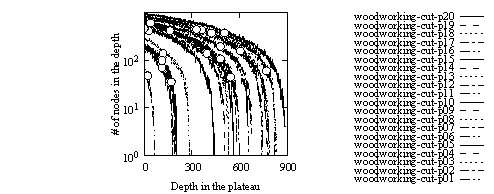
\includegraphics{tables/aaai16-log-rd/2zerocost/depth-histogram-lmcut_rdlog1-woodworking-cut.pdf}
 \caption{Histogram of the depths in the plateau in
\pddl{Woodworkin-cut} instances using $[h,\rd,\ro]$. $y$ axis is logarithmic.
 Large dots show where the solutions were found.
 }
 \label{depth-histogram}
\end{figure}


\subsubsection{Is Depth-based Tie-breaking Necessary?}
% is this the right location -- maybe this should in a discussion section?


\begin{table}[tb]
 \setlength{\tabcolsep}{0.3em}
 \centering \relsize{-1}
 \begin{tabular}{|c||c|c||c|}
\hline         
 Domain & \rotatebox[origin=l]{90}{$[h,\ro]$}   & \rotatebox[origin=l]{90}{$[h,\rd,\ro]$}   & \rotatebox[origin=l]{90}{$[h,\ro]$}\rotatebox[origin=l]{90}{$[h,\rd,\ro]$}    \\
\hline         
 sum(1104) &  559.8\spm{}1.0 &  570.6\spm{}1.5 &  0.0  \\
\hline         
 {\relsize{-1}cybersec(19)} &  4.4\spm{}1.0 &  9.6\spm{}1.1 &  0.0  \\
 {\relsize{-1}openstacks-opt11(20)} &  11.6\spm{}0.5 &  18.0\spm{}0.0 &  0.0  \\
 {\relsize{-1}pipesworld-notankage(50)} &  14.9\spm{}0.3 &  14.2\spm{}0.4 &  0.0 \\\hline
 sum(640) &  279.9\spm{}1.8 &  302.2\spm{}2.4 &  0.0  \\
\hline         
 {\relsize{-1}elevators-up(20)} &  7.3\spm{}0.5 &  9.4\spm{}1.1 &  0.0  \\
 {\relsize{-1}freecell-move(20)} &  5.0\spm{}0.4 &  16.5\spm{}0.7 &  0.0  \\
 {\relsize{-1}gripper-move(20)} &  7.0\spm{}0.0 &  6.0\spm{}0.0 &  0.0  \\
 {\relsize{-1}logistics00-fuel(28)} &  16.0\spm{}0.0 &  15.0\spm{}0.0 &  0.0  \\
 {\relsize{-1}miconic-up(30)} &  17.0\spm{}0.4 &  19.8\spm{}1.0 &  0.0  \\
 {\relsize{-1}mprime-succumb(35)} &  17.9\spm{}0.5 &  20.1\spm{}0.7 &  0.0  \\
 {\relsize{-1}pipesnt-pushstart(20)} &  8.5\spm{}0.5 &  9.8\spm{}0.4 &  0.0  \\
 {\relsize{-1}tpp-fuel(30)} &  8.1\spm{}0.3 &  11.0\spm{}0.0 &  0.0  \\
 {\relsize{-1}woodworking-cut(20)} &  7.1\spm{}0.3 &  8.6\spm{}0.9 &  0.0 \\\hline
 total(1744) &  839.7\spm{}2.1 &  872.8\spm{}2.9 &  0.0 \\\hline
\end{tabular}

 \caption{Performance of RandomOrder last-level tiebreaking with/without RandomDepth tie-breaking. Each cell
 shows the coverage (mean $\pm$ sd) on each domain (5min, 2GB)$\times$10 runs. 
Due to space, only domains with results 
 significantly different results  (according to the Wilcoxon test, $p<0.05$) are shown.
See supplement for full results.
 }  \label{r-vs-rd-random}
\end{table}

We have shown that $[h,\rd,\ro]$ performs well overall, but
one might wonder whether the power of this strategy really comes from depth-based tie-breaking, or from randomness.
\reftbl{r-vs-rd-random} shows that $[h,\ro]$ performs poorly, so clearly, random tie-breaking combined with $h$-based tie-breaking is not sufficient.
The reason that $[h,\ro]$ performs so poorly is that if we select uniformly from a the bucket of all open nodes in the plateau, there is a very strong bias for selecting a node with low depth, simply because at any given point during the search in the plateau region, more nodes closer to the entrance of the plateau (i.e., lower depth) will have been generated.
By randomly selecting a depth bucket, $[h,\rd,\ro]$ explicitly eliminates this bias for selecting nodes for low depth.

% COMMENTED OUT: random-h is too weak, because if we have an admissible heuristic, the adversary can't fool h.
% One might also wonder whether the power of $[h,\rd,\ro]$ comes from having multiple levels of randomness, and not from the notion of depth.
% This is not the case -- multiple levels of randomness would not suffice to capture the power of $[h,\rd,\ro]$ due to the following reason:
% Consider another possible randomized strategy, $[random-h,\ro]$, which first picks a random $h$-bucket, 
% and then picks a random element from that bucket.
% When the final plateau of [f,h] is small, tie-breaking strategies do not significantly affect performance.
% However, when the final plateau of [f,h] is large, then $[random-h,\ro]$ will behave similarly to $[h,\ro]$, because almost all nodes in the search space have the same h-value, and we have shown that $[h,\ro]$ performs poorly on domains with large plateaus, i.e., domains with zero-cost-actions., compared to $[h,\rd,\ro]$.
% Thus, multiple levels of randomness alone do not account for the success of $[h,\rd,\ro]$, and the notion of depth buckets seems necessary.


\section{Domain-Configuration and Tie-Breaking}
%Moved this out of the depth-based evaluation section because we also evaluate [h,fifo] and [h,lifo], and the results show that all are robust wrto actin ordering
Recently, \citeauthor{vallati2015effective} showed that the performance of 
satisficing planners was significantly affected by PDDL domain \emph{configurations}, which includes the name/ordering of actions, propositions, and objects in the PDDL input file (\citeyear{vallati2015effective}).
% note that vallati et al did not show that tie-breaking was affected -- they observed that performance of the planners was affected by configuration, and conjectured that the performance variation was due to the effects of configuration on tie-breaking.
They conjectured that performance variations caused
by different domain configurations is due to the impact that the naming/ordering of objects has on tie-breaking.
% in \cite{vallati2015effective} p.7, col2, par#1
In Fast Downward, action names can affect search performance, because FD 
sorts the action schemas according to the dictionary
order of the schema names, which affects the order of applicable ground
actions, which in turn affects the order in which nodes
are inserted into OPEN.

%%%%%%%%%%%%%%%%%%%%%%%%%%%%%%%%%%%%%%%%%%%%%%%%%%%%5

We tested the robustness of the standard $[h,\lifo]$ and $[h,\fifo]$ strategies, as well as $[h,\rd,\ro]$,
with respect to 
biases introduced by domain configuration (action naming) in the PDDL domain definition.
We created 3 different sets of domains in which the
original names of action schema are mangled into random strings. 
%We only reordered the actions becasue in the FD codebase, the order of propositions has no effect on tie-breaking. --- let's avoid talking about anything other than action names, in case there are other configuration factors.
%  XXXTODO CHECK whether above sentence correctly summarizes the sentence below.
%% In contrast, we continued to use the variable ordering in the original domains
%% because the effect of variable ordering is irrelevant to the tie-breaking
%% criteria.
% %We avoided the effect of action orderings by using the randomized third tie-breakings.
%Each set of action-renamed domains contains all of the benchmark and zerocost domains.   %XX - can be inferred from table
We ran each of the 3 strategies on each
set of mangled domains, three times each with different random seeds,
resulting in 9 runs per strategy (recall that robustness wrto random seed was shown in \refsec{sec:depth-based-evaluation}.)

The results are shown in \reftbl{actionordering-robustness} (We
also included the original 10 runs from  \reftbl{depth}).
We statistically analysed the results for $[h,\rd,\ro]$ 
to see if any of the 4 sets of domains
significantly outperformed the others.
%In order to test the significance of mean value,
We first applied Fligner-Killeen's non-parametric test to see if the sample groups 
in each set of randomized domains share the same variance, 
but could not reject the homogeneity of variances ($p=0.74$).
Since the variances were not significantly different,
we could then apply the non-parametric Kruskal-Wallis test to see if
there is any difference in the mean values between the original
population of the sample groups, which showed that the differences were not significant ($p=0.26$),
i.e., action name mangling did not significnatly affect performance.

Thus, in contrast to the results for satisficing search by \cite{vallati2015effective}, 
the effect of action ordering  seems to be relatively weak for cost-optimal search using \astar.
This may be because 
compared to the satisficing, best-first serach algorithms evaluated in \cite{vallati2015effective},
the behavior of $[h,\lifo]$, $[h,\fifo]$, and $[h,rd,\ro]$ highly
constrained, because of the first-level tie-breaking according to $h$.
%in that all nodes with cost $f$ must be expanded before any nodes with cost larger than $f$. % this is true for best-first-search in general, by definition.

\begin{table}[tb]
 \setlength{\tabcolsep}{0.2em}
 \centering \relsize{-1}
 %\begin{tabular}{|c||c|c||c|c|c||c|c|c||c|c|c||c|c|c|}
\hline                                          
 Domain & \rotatebox[origin=l]{90}{lmcut,ld,randomx}   & \rotatebox[origin=l]{90}{lmcut,rd,randomx}   & \rotatebox[origin=l]{90}{lmcut,ld,randomx,2280}   & \rotatebox[origin=l]{90}{lmcut,ld,randomx,2432}   & \rotatebox[origin=l]{90}{lmcut,ld,randomx,15314}   & \rotatebox[origin=l]{90}{lmcut,rd,randomx,2280}   & \rotatebox[origin=l]{90}{lmcut,rd,randomx,2432}   & \rotatebox[origin=l]{90}{lmcut,rd,randomx,15314}   & \rotatebox[origin=l]{90}{lmcut,ld,randomx,2280}   & \rotatebox[origin=l]{90}{lmcut,ld,randomx,2432}   & \rotatebox[origin=l]{90}{lmcut,ld,randomx,15314}   & \rotatebox[origin=l]{90}{lmcut,rd,randomx,2280}   & \rotatebox[origin=l]{90}{lmcut,rd,randomx,2432}   & \rotatebox[origin=l]{90}{lmcut,rd,randomx,15314}    \\
\hline                                          
 sum(1104) &  568.0\spm{}1.4 &  571.7\spm{}0.9 &  567 &  567 &  570 &  571 &  573 &  571 &  53453876429 &  53453445617 &  53153939944 &  53054630959 &  52855052463 &  53055118088 \\\hline
 sum(380) &  172.7\spm{}2.1 &  169.7\spm{}0.5 &  173 &  175 &  170 &  170 &  169 &  170 &  20745209155 &  20554935065 &  21038450133 &  21044249397 &  21139379995 &  21045425987 \\\hline
 sum(260) &  130.0\spm{}2.8 &  127.0\spm{}0.8 &  126 &  132 &  132 &  128 &  126 &  127 &  13135650022 &  12538926357 &  12539913452 &  12953782527 &  13146086022 &  13041215376 \\\hline
 sum(1104) &  568.0\spm{}1.4 &  571.7\spm{}0.9 &  567 &  567 &  570 &  571 &  573 &  571 &  53154445513 &  53154525092 &  53353719312 &  52954806534 &  52954410880 &  53154246049 \\\hline
 sum(380) &  172.7\spm{}2.1 &  169.7\spm{}0.5 &  173 &  175 &  170 &  170 &  169 &  170 &  20745376136 &  20555172324 &  21038588895 &  20845700303 &  20744544273 &  20742668307 \\\hline
 sum(260) &  130.0\spm{}2.8 &  127.0\spm{}0.8 &  126 &  132 &  132 &  128 &  126 &  127 &  13325387377 &  12331490437 &  12830251681 &  12555898212 &  13138649739 &  12267203886 \\\hline
 sum(1104) &  568.0\spm{}1.4 &  571.7\spm{}0.9 &  567 &  567 &  570 &  571 &  573 &  571 &  53154844965 &  53154545412 &  53054498298 &  52854208990 &  52654902163 &  53054545808 \\\hline
 sum(380) &  172.7\spm{}2.1 &  169.7\spm{}0.5 &  173 &  175 &  170 &  170 &  169 &  170 &  20745213348 &  20554939144 &  21038454659 &  20941436904 &  20941330432 &  20857182304 \\\hline
 sum(260) &  130.0\spm{}2.8 &  127.0\spm{}0.8 &  126 &  132 &  132 &  128 &  126 &  127 &  13227678250 &  12531692255 &  12831380301 &  12952354353 &  12761488656 &  12948386130 \\\hline
\end{tabular}

 %\begin{tabular}{|c||c|c|c||c|c|c|}
\hline                  
 Domain & \rotatebox[origin=l]{90}{lmcut,rd,randomx,2280}   & \rotatebox[origin=l]{90}{lmcut,rd,randomx,2432}   & \rotatebox[origin=l]{90}{lmcut,rd,randomx,15314}   & \rotatebox[origin=l]{90}{lmcut,rd,randomx,2280}   & \rotatebox[origin=l]{90}{lmcut,rd,randomx,2432}   & \rotatebox[origin=l]{90}{lmcut,rd,randomx,15314}    \\
\hline                  
 sum(1104) &  571 &  573 &  571 &  53054630959 &  52855052463 &  53055118088 \\\hline
 sum(1104) &  571 &  573 &  571 &  52954806534 &  52954410880 &  53154246049 \\\hline
 sum(1104) &  571 &  573 &  571 &  52854208990 &  52654902163 &  53054545808 \\\hline
 sum(380) &  170 &  169 &  170 &  21044249397 &  21139379995 &  21045425987 \\\hline
 sum(380) &  170 &  169 &  170 &  20845700303 &  20744544273 &  20742668307 \\\hline
 sum(380) &  170 &  169 &  170 &  20941436904 &  20941330432 &  20857182304 \\\hline
 sum(260) &  128 &  126 &  127 &  12953782527 &  13146086022 &  13041215376 \\\hline
 sum(260) &  128 &  126 &  127 &  12555898212 &  13138649739 &  12267203886 \\\hline
 sum(260) &  128 &  126 &  127 &  12952354353 &  12761488656 &  12948386130 \\\hline
\end{tabular}

 %\begin{tabular}{|c||c|c|c||c|c|c|}
\hline                  
 Domain & \rotatebox[origin=l]{90}{lmcut,rd,randomx,2280}   & \rotatebox[origin=l]{90}{lmcut,rd,randomx,2432}   & \rotatebox[origin=l]{90}{lmcut,rd,randomx,15314}   & \rotatebox[origin=l]{90}{lmcut,rd,randomx,2280}   & \rotatebox[origin=l]{90}{lmcut,rd,randomx,2432}   & \rotatebox[origin=l]{90}{lmcut,rd,randomx,15314}    \\
\hline                  
 sum(1104) &  571 &  573 &  571 &  53054630959 &  52855052463 &  53055118088 \\\hline
 sum(1104) &  571 &  573 &  571 &  52954806534 &  52954410880 &  53154246049 \\\hline
 sum(1104) &  571 &  573 &  571 &  52854208990 &  52654902163 &  53054545808 \\\hline
 sum(380) &  170 &  169 &  170 &  21044249397 &  21139379995 &  21045425987 \\\hline
 sum(380) &  170 &  169 &  170 &  20845700303 &  20744544273 &  20742668307 \\\hline
 sum(380) &  170 &  169 &  170 &  20941436904 &  20941330432 &  20857182304 \\\hline
 sum(260) &  128 &  126 &  127 &  12953782527 &  13146086022 &  13041215376 \\\hline
 sum(260) &  128 &  126 &  127 &  12555898212 &  13138649739 &  12267203886 \\\hline
 sum(260) &  128 &  126 &  127 &  12952354353 &  12761488656 &  12948386130 \\\hline
\end{tabular}

 \begin{tabular}{|c|c|c||c|}
\hline         
 Domain & $[h,\fifo]$ & $[h,\lifo]$   & \spc{$[h,\rd,\ro]$ \\($n$: number of runs)}    \\
\hline         
 Mangled IPC 1 (1104) &  556 &  564 &  571.7\spm{}0.9 ($n=3$)\\\hline
 Mangled IPC 2 (1104) &  557 &  568 &  571.3\spm{}0.9 ($n=3$)\\\hline
 Mangled IPC 3 (1104) &  557 &  568 &  573.0\spm{}1.6 ($n=3$)\\\hline
 Original IPC (1104) &  558 &  565 &  570.6\spm{}1.5 ($n=10$)\\\hline
 Mangled Zerocost 1 (620) &  256 &  277 &  288.7\spm{}3.7 ($n=3$)\\\hline
 Mangled Zerocost 2 (620) &  256 &  277 &  285.0\spm{}0.8 ($n=3$)\\\hline
 Mangled Zerocost 3 (620) &  256 &  279 &  286.7\spm{}0.9 ($n=3$)\\\hline
 Original Zerocost  (620) &  256 &  279 &  287.2\spm{}2.4 ($n=10$)\\\hline
\end{tabular}

 \caption{Results showing the total coverages of $[h,\fifo]$, $[h,\lifo]$
 and $[h,\rd,\ro]$ with three seeds. Each row represents the original set of
 domains or its three action-reordered variants. The effect
 of action ordering is small enough for $[h,\rd,\ro]$ to
 constantly perform better than the traditional tiebreaking methods.}
 \label{actionordering-robustness}
\end{table}

\section{Related Work}
\label{sec-4}

Previous work on escaping search space plateaus has focused on
non-admissible search.  DBFS \cite{imai2011novel} is a technique which
adds stochastic backtracking to Greedy Best First Search to avoid
being misdirected by the heuristic function. Type based bucket
\cite{xie14type} classifies the plateau of GBFS according to the
$[g,h]$ pair and distributes the effort.  Marvin \cite{Coles07} learns plateau-escaping macros
from the Enhanced Hill Climbing phase of the FF planner
\cite{Hoffmann01} and later uses these macros to escape the plateau.
\citeauthor{Hoffmann05} gives a detailed analysis of the
structure of the search space in the benchmark domains which were
available in \citeyear{Hoffmann05} \cite{Hoffmann05,Hoffmann14}. 
The analysis was focused on the plateaus and dead ends which occur during the inadmissible search.
% 
However, to our knowledge, searching in plateaus has not been
previously investigated for cost-optimal planning with admissible
search.
The meaning of plateau in inadmissible and admissible search are
different in how to treat the non-final plateaus: Inadmissible search can
skip or escape a plateau whenever possible, while
admissible search cannot skip the remaining nodes in a plateau unless it
is the final plateau and it directly finds a solution.

%In their work on combining multiple heuristics in a planner, 
\citeauthor{RogerH10} (\citeyear{RogerH10}) considered a tie-breaking approach which works as follows:
When combining two heuristics, one of the
heuristics is used as the primary criterion for guiding the search,
and the second heuristic is used to break ties among nodes with the same primary
heuristic value.
While this did not perform well in their work on satisficing planning, 
using a secondary heuristic as a tie-breaking criterion in our multi-level tie-breaking framework 
for cost-optimal search is an interesting direction for future work.

The PLUSONE %\footnote{This term is used on the Fast Downward website.} XXfootnote takes too much space
cost-type is a non-admissible search technique in the Fast Downward/LAMA planner
\cite{richter2010lama} which increases all action costs by 1.
By eliminating zero-cost actions, this has the effect similar to our
FirstDepth tie-breaking.
%Using PLUSONE, three successive
%applications of zero-cost operators have cost 3, and two
%applications have cost 2, and smaller cost is preferred, just as
%\astar always expands the node with smaller $f$-value.
This technique explicitly targeted zero-cost actions,
and resulted in a significantly better performance in IPC-6
satisficing track \cite[p.137, Sec. 3.3.2]{richter2010lama}.
\todo*{citation}
% There's a long discussion of Openstacks in \cite{richter2010lama}, p.167-169, but I can't find PLUSONE anywhere. Maybe it's called something else in the paper?  Maybe \richter2010lama is the wrong citation??
Unlike PLUSONE, depth-based tie-breaking is admissible.
%because unlike PLUSONE, action costs are not modified.  
Also, \emph{we
do not always favor smaller depth over larger depth}. LAMA treats the
increased cost as the part of sorting criteria and always prefers
smaller cost, much like in our FirstDepth strategy.  However, FirstDepth
strategy is the worst strategy in our experiments and the best
performing depth-based tie-breaking methods are LastDepth and RandomDepth
in our experiments, and they do not prefer the smaller depth.

% It's not clear what these techniques have in common, except that they are all orthogonal to heuristics,
% If that's the case, then there's no need to cite them in this paper -- there's no reason why these particular techniques
% are more relevant to this paper than hundreds of other techniques that are orthogonal to heuristics.
%% In admissible planning,
%% \emph{Symmetry Breaking}
%% \cite{Fox1998,pochter2011exploiting,domshlak2013symmetry} is the search
%% technique that tries to prune the states with symmetric
%% paths. \emph{Partial Order Reduction}
%% % , \emph{Strong Stubbern Sets} and \emph{Expansion Core} are
%% is also a technique which prunes the
%% intermediate states that reach to the same goal using the different
%% orders of same actions. \emph{Dominance Pruning} \cite{hall2013faster} is a
%% technique which prunes a state if it can be proven to be worse than the other nodes.
%% % 
%% These are usually not considered an attempt to improve the heuristic
%% estimates, however, in terms of \emph{Path-dependent globally admissible
%% heurisitics} \cite{karpas2012optimal}, a class of heuristics which is
%% admissible only on a particular optimal path, generalizes the above
%% techniques as assigining an infinite cost to some nodes on the other optimal paths.
%% % 
%% % From a slightly different category, Pathmax \cite{mero1984heuristic} and
%% % Bidirectional Pathmax \cite{felner2011inconsistent} are the techniques
%% % which converts an inconsistent heuristics into non-decreasing,
%% % consistent heuristics.
%% Thus, in a broad term, all of these methods are the
%% attempts to improve the heuristic estimates.
%% % Although in some particular
%% % case they may be able to return a perfect heuristics, they are still not
%% % always a perfect heuristics, implying that the plateau is unavoidable.
%% In contrast, our tie-breaking techniques aims specifically at the case
%% where the plateau is encountered and the planners are forced to run a
%% knowledge-free search.

$LA^*$ \cite{stern2010look} extends \astar by performing a
cost-bounded depth-first \emph{lookahead} from each node as it is generated.
%Although this work was not done in the context of tie-breaking strategies, it is interesting to note that 
when the lookahead cost bound $k=0$ ($LA^*_0$ in their notation), only nodes with the same $f$-value as the current \astar frontier are expanded, which corresponds to a LastDepth tie-breaking strategy.


\section{Conclusion}

In this paper, we evaluated standard tie-breaking
strategies for \astar, and proposed a simple,
depth-based, randomized strategy $[h,\rd,\ro]$, which 
significantly outperforms previous strategies on domains with zero-cost actions, 
and slightly outperforms previous strategies on benchmark problems without zero-cost actions.
Although we only showed results on a planner using the LM-cut heuristic due to space, 
results were similar using the M\&S heuristic  (please see Supplement), so our results regarding tie-breaking are consistent when using different heuristic functions.

Our approach is effective on domains where zero-cost actions create large plateau regions where all nodes have the same $f$ and $h$ costs
and the heuristic function provides no useful guidance.
We argued that such domains arise naturally when considering resource optimization problems.

It also avoids the effect of action ordering in the domain definition,
providing a robust behavior.

 % when the distribution of optimal solutions is not uniform within the open list.
% We also showed that this nonuniform distribution still appears when we have almost-perfect % heuristics.

Our method differs from the pruning techniques because we do not prune
any states, nor from the other general improvements to the heuristic
accuracy because we just change the evaluation order within the same
$f$, yet it address the fundamental problems in the heuristic forward
search. 
% 
Future work includes a development of learning technique for
adaptively altering the search behavior in the plateau.



